% ******************************* Thesis Appendix B ********************************

\chapter{TRECVID MED 2014 Results}

\ifpdf
\graphicspath{{Appendix2/Figs/Raster/}{Appendix2/Figs/PDF/}{Appendix2/Figs/}}
\else
\graphicspath{{Appendix2/Figs/Vector/}{Appendix2/Figs/}}
\fi

In MED 2014, we study some technical improvements for motion feature and image features over our MED 2014 System.

\section{For Motion Feature}
We use the improved version of Dense Trajectories motion feature \cite{wang2013action}. To describe trajectories, we choose to use both HOGHOF and MBH descriptors, which have been proved to be effective for MED by AXES team \cite{aly2013axes}. In order to combine these descriptors, we train two independent GMM codebooks. After that Fisher vector is used to encode feature from each descriptor independently. The resulting representation at video level of each descriptor is normalized by power normalization and L2 normalization. Finally these two feature vectors are concatenated to form the final representation of each video.

\section{For Image Feature}
We apply two technical improvements on the image feature. At first, a new way of video level feature representation is used to pool feature from its keyframe-based representation. In MED 2013 system, we aggregated local descriptors from all sampled frames in video without explicitly calculating keyframe-based features. For this year's system, Fisher vector is encoded for each sampled frame and normalized using power and L2 normalization. Features from these sampled frames are averaged to form the video level representation. The second technical improvement is using RootSIFT features \cite{arandjelovic2012three}. We have applied RootSIFT with different implementation of SIFT features such as the one use in \cite{mikolajczyk2005performance}, VLFeat \cite{vedaldi08vlfeat}, and Color Descriptor \cite{vandeSandeTPAMI2010}. Finally we chose to use VLFeat because it achieved the best performance in our evaluation framework.

We evaluated the performance of new components on the KINDREDTEST 13 dataset. All results are reported in terms of Mean Average Precision (MAP). Performance comparison of motion features and image features are shown in Table \ref{t_motion} and Table \ref{t_sift} respectively. 

\begin{table}
	\renewcommand{\arraystretch}{1.3}	
	\caption{Performance comparison of different motion feature configurations.}
	\label{t_motion}
	\centering
	\begin{tabular}{cccll}
		\cline{1-3}
		\multicolumn{1}{|c|}{MED13 System}                                                       & \multicolumn{2}{c|}{MED14 System}                                                                                                                                                                            &  &  \\ \cline{1-3}
		\multicolumn{1}{|c|}{\begin{tabular}[c]{@{}c@{}}Dense Trajectories\\ (MBH)\end{tabular}} & \multicolumn{1}{c|}{\begin{tabular}[c]{@{}c@{}}Improved Dense \\ Trajectories (MBH)\end{tabular}} & \multicolumn{1}{c|}{\begin{tabular}[c]{@{}c@{}}Improved Dense \\ Trajectories (HOGHOF + MBH)\end{tabular}} &  &  \\ \cline{1-3}
		\multicolumn{1}{|c|}{28.33}                                                              & \multicolumn{1}{c|}{35.07}                                                                       & \multicolumn{1}{c|}{40.77}                                                                                &  &  \\ \cline{1-3}
		\multicolumn{1}{l}{}                                                                     & \multicolumn{1}{l}{}                                                                             & \multicolumn{1}{l}{}                                                                                      &  & 
	\end{tabular}
\end{table}
\begin{table}
	\renewcommand{\arraystretch}{1.3}
	\renewcommand{\arraystretch}{1.3}	
	\caption{Performance comparison of different image feature configurations.}
	\label{t_sift}
	\centering
	\begin{tabular}{cccll}
		\cline{1-3}
		\multicolumn{1}{|c|}{MED13 System} & \multicolumn{2}{c|}{MED14 System}                                                                                                                                                        &  &  \\ \cline{1-3}
		\multicolumn{1}{|c|}{SIFT}         & \multicolumn{1}{c|}{\begin{tabular}[c]{@{}c@{}}SIFT\\ (New aggregation)\end{tabular}} & \multicolumn{1}{c|}{\begin{tabular}[c]{@{}c@{}}SIFT\\ (New aggregation + RootSIFT)\end{tabular}} &  &  \\ \cline{1-3}
		\multicolumn{1}{|c|}{23.41}        & \multicolumn{1}{c|}{24.24}                                                            & \multicolumn{1}{c|}{27.02}                                                                       &  &  \\ \cline{1-3}
		\multicolumn{1}{l}{}               & \multicolumn{1}{l}{}                                                                  & \multicolumn{1}{l}{}                                                                             &  & 
	\end{tabular}
\end{table}

Unfortunately, we could not finish running the best configuration for motion features, so we use the same configuration as previous year because it took less time. For image feature, we used the improved version. We also used the late fusion technique to combine audio and visual features in our final submission. For related videos, we fixed our system to use them as negative training samples for both EK10 and EK100 settings. We participated in the full evaluation set containing around 200K videos for both Pre-specified (PS) and Adhoc (AH) tasks.

\section{Results and Conclusion} 
Results of our MED system is shown in Fig. \ref{fig:results}. Our ranks was 11th out of 12 teams in the EK10 setting and 10th in the EK100 setting. This observation is same for both PS and AH tasks. Compared to top MED systems, our system is significantly worse in the EK10 setting. For example, our performance are 67\% and 41\% relatively to the best MED system in the EK100 and EK10 respectively. We have learnt that top performance system have incorporated semantic concept detection, which can be more helpful when number of training videos are limited. This might be the reason for the significant drop on the performance of our EK10 system.

\begin{figure}
	\centering
	\begin{subfigure}{\textwidth}
		\centering
		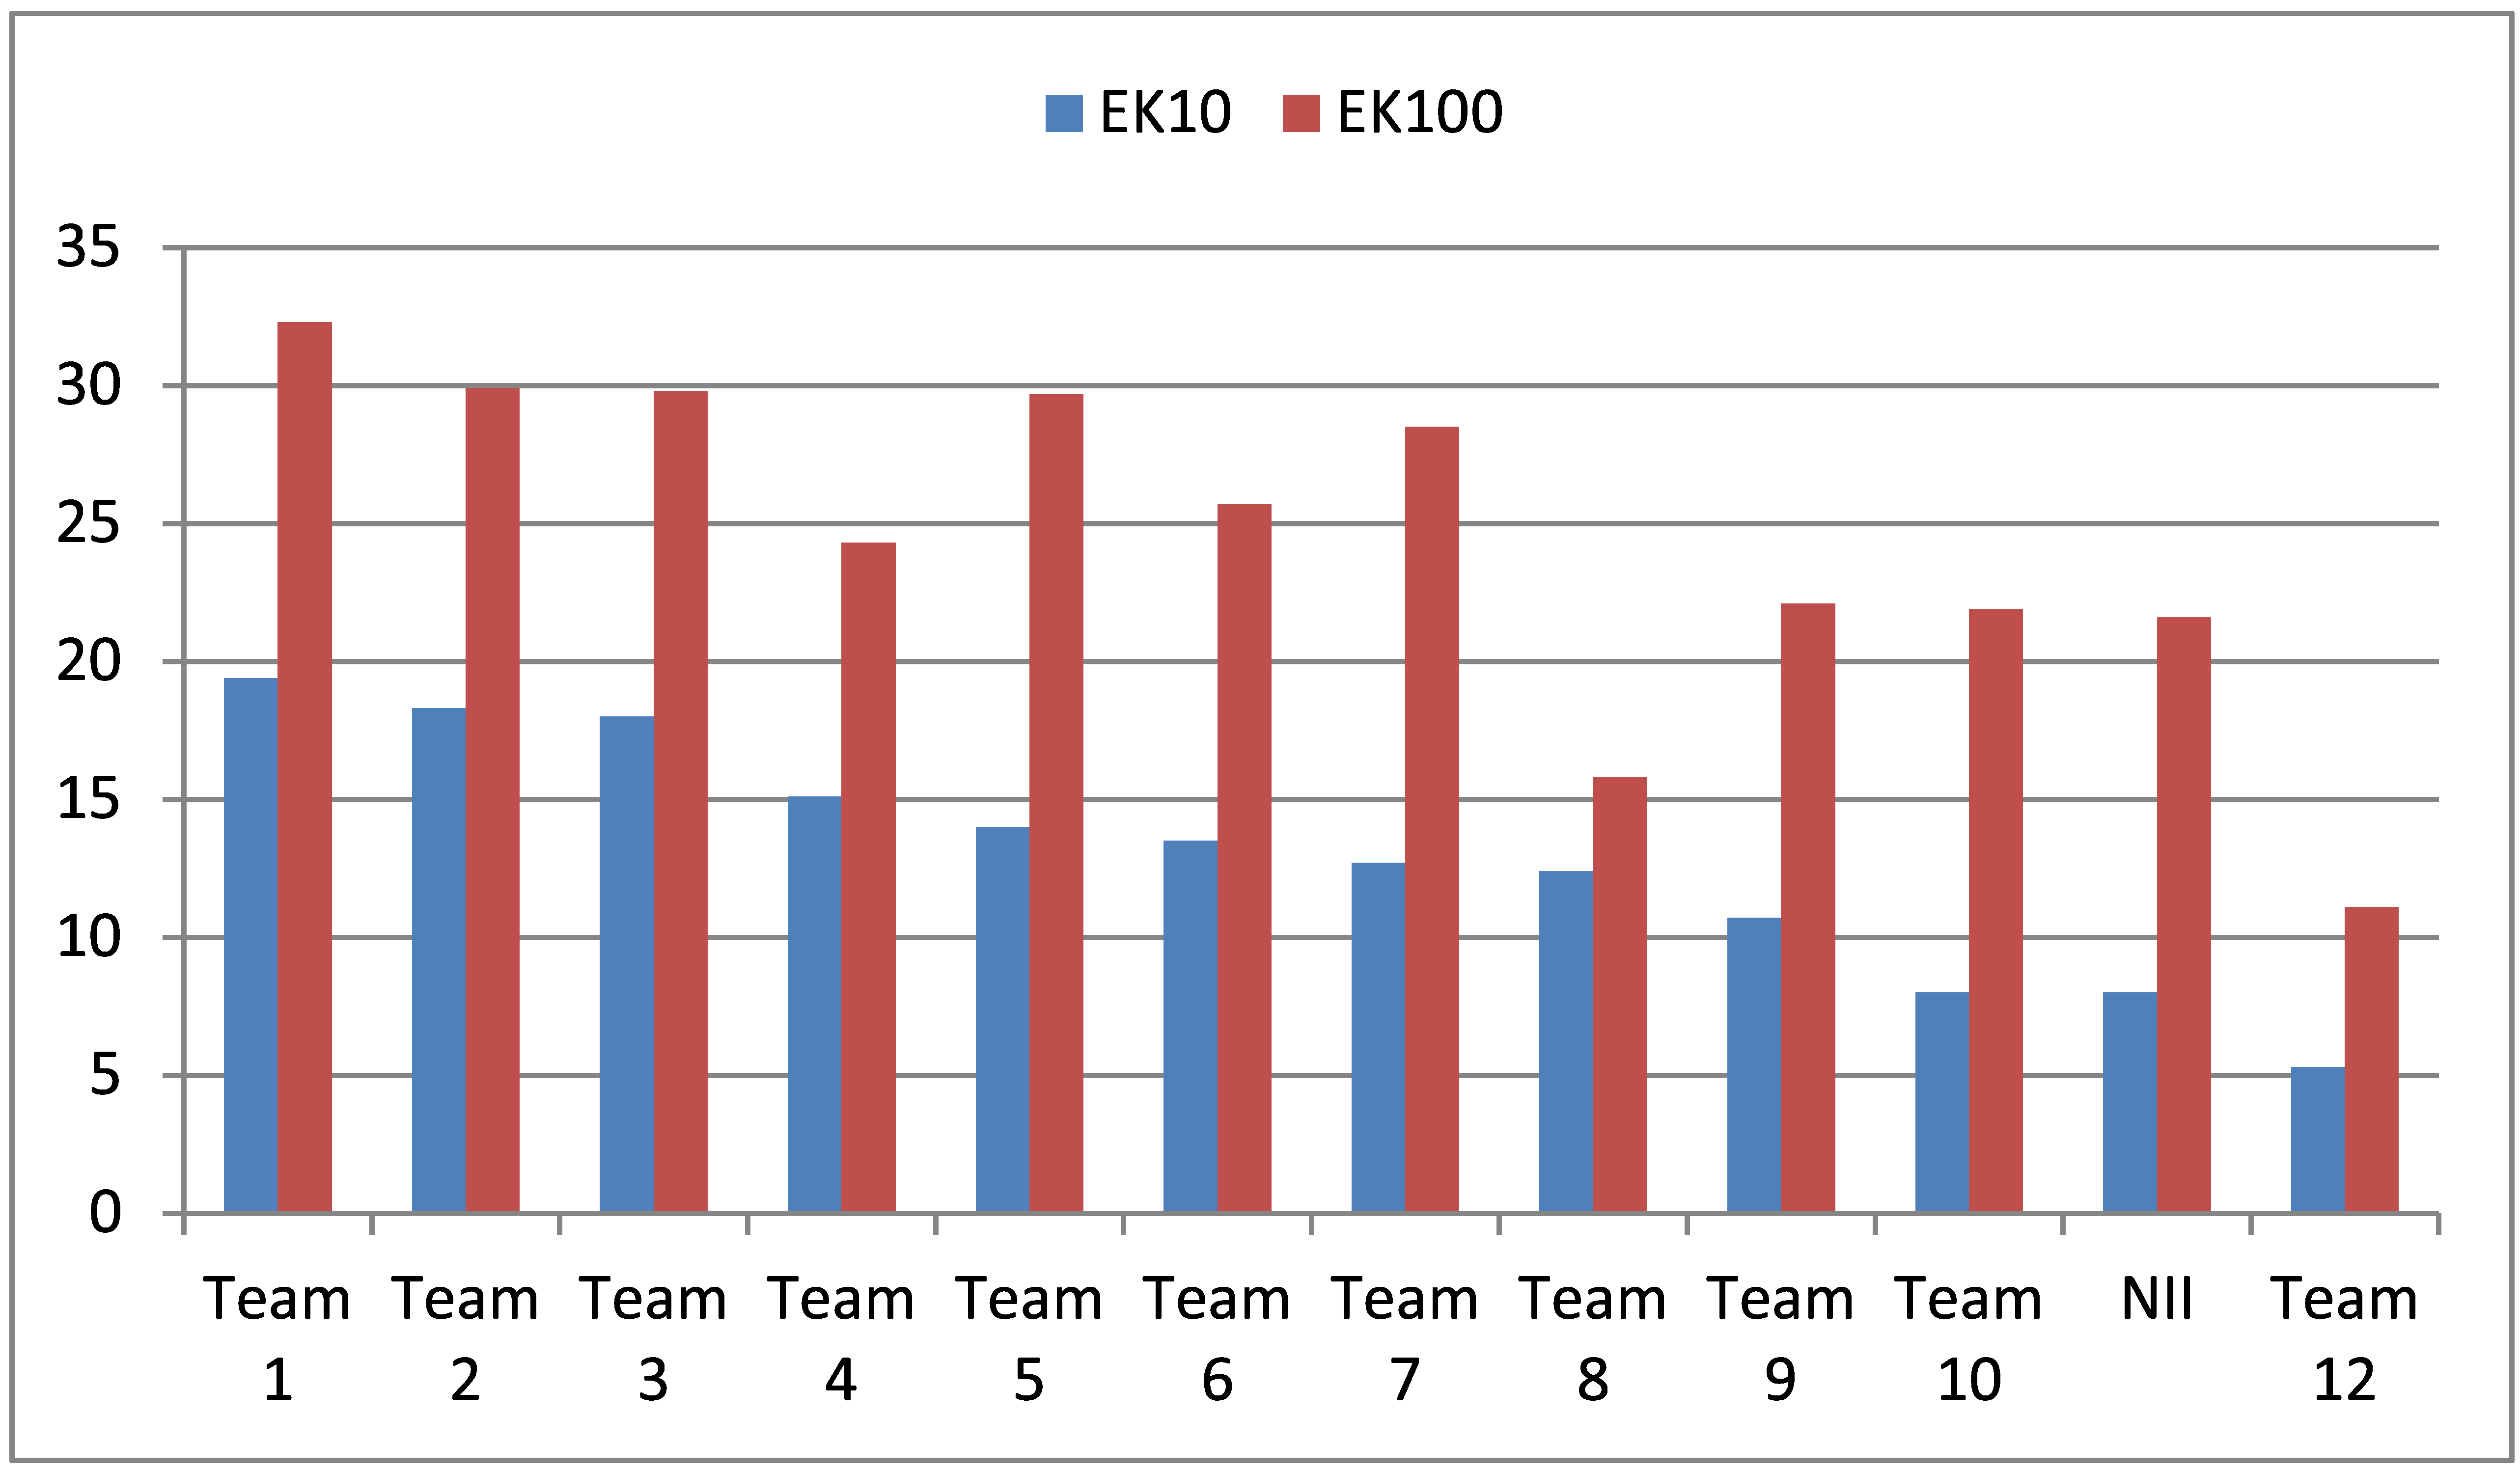
\includegraphics[width=0.7\linewidth]{med_result_ps.pdf}
		\caption{Pre-Specified systems}
		\label{fig_result_ps}
	\end{subfigure} 
	\begin{subfigure}{\textwidth}
		\centering
		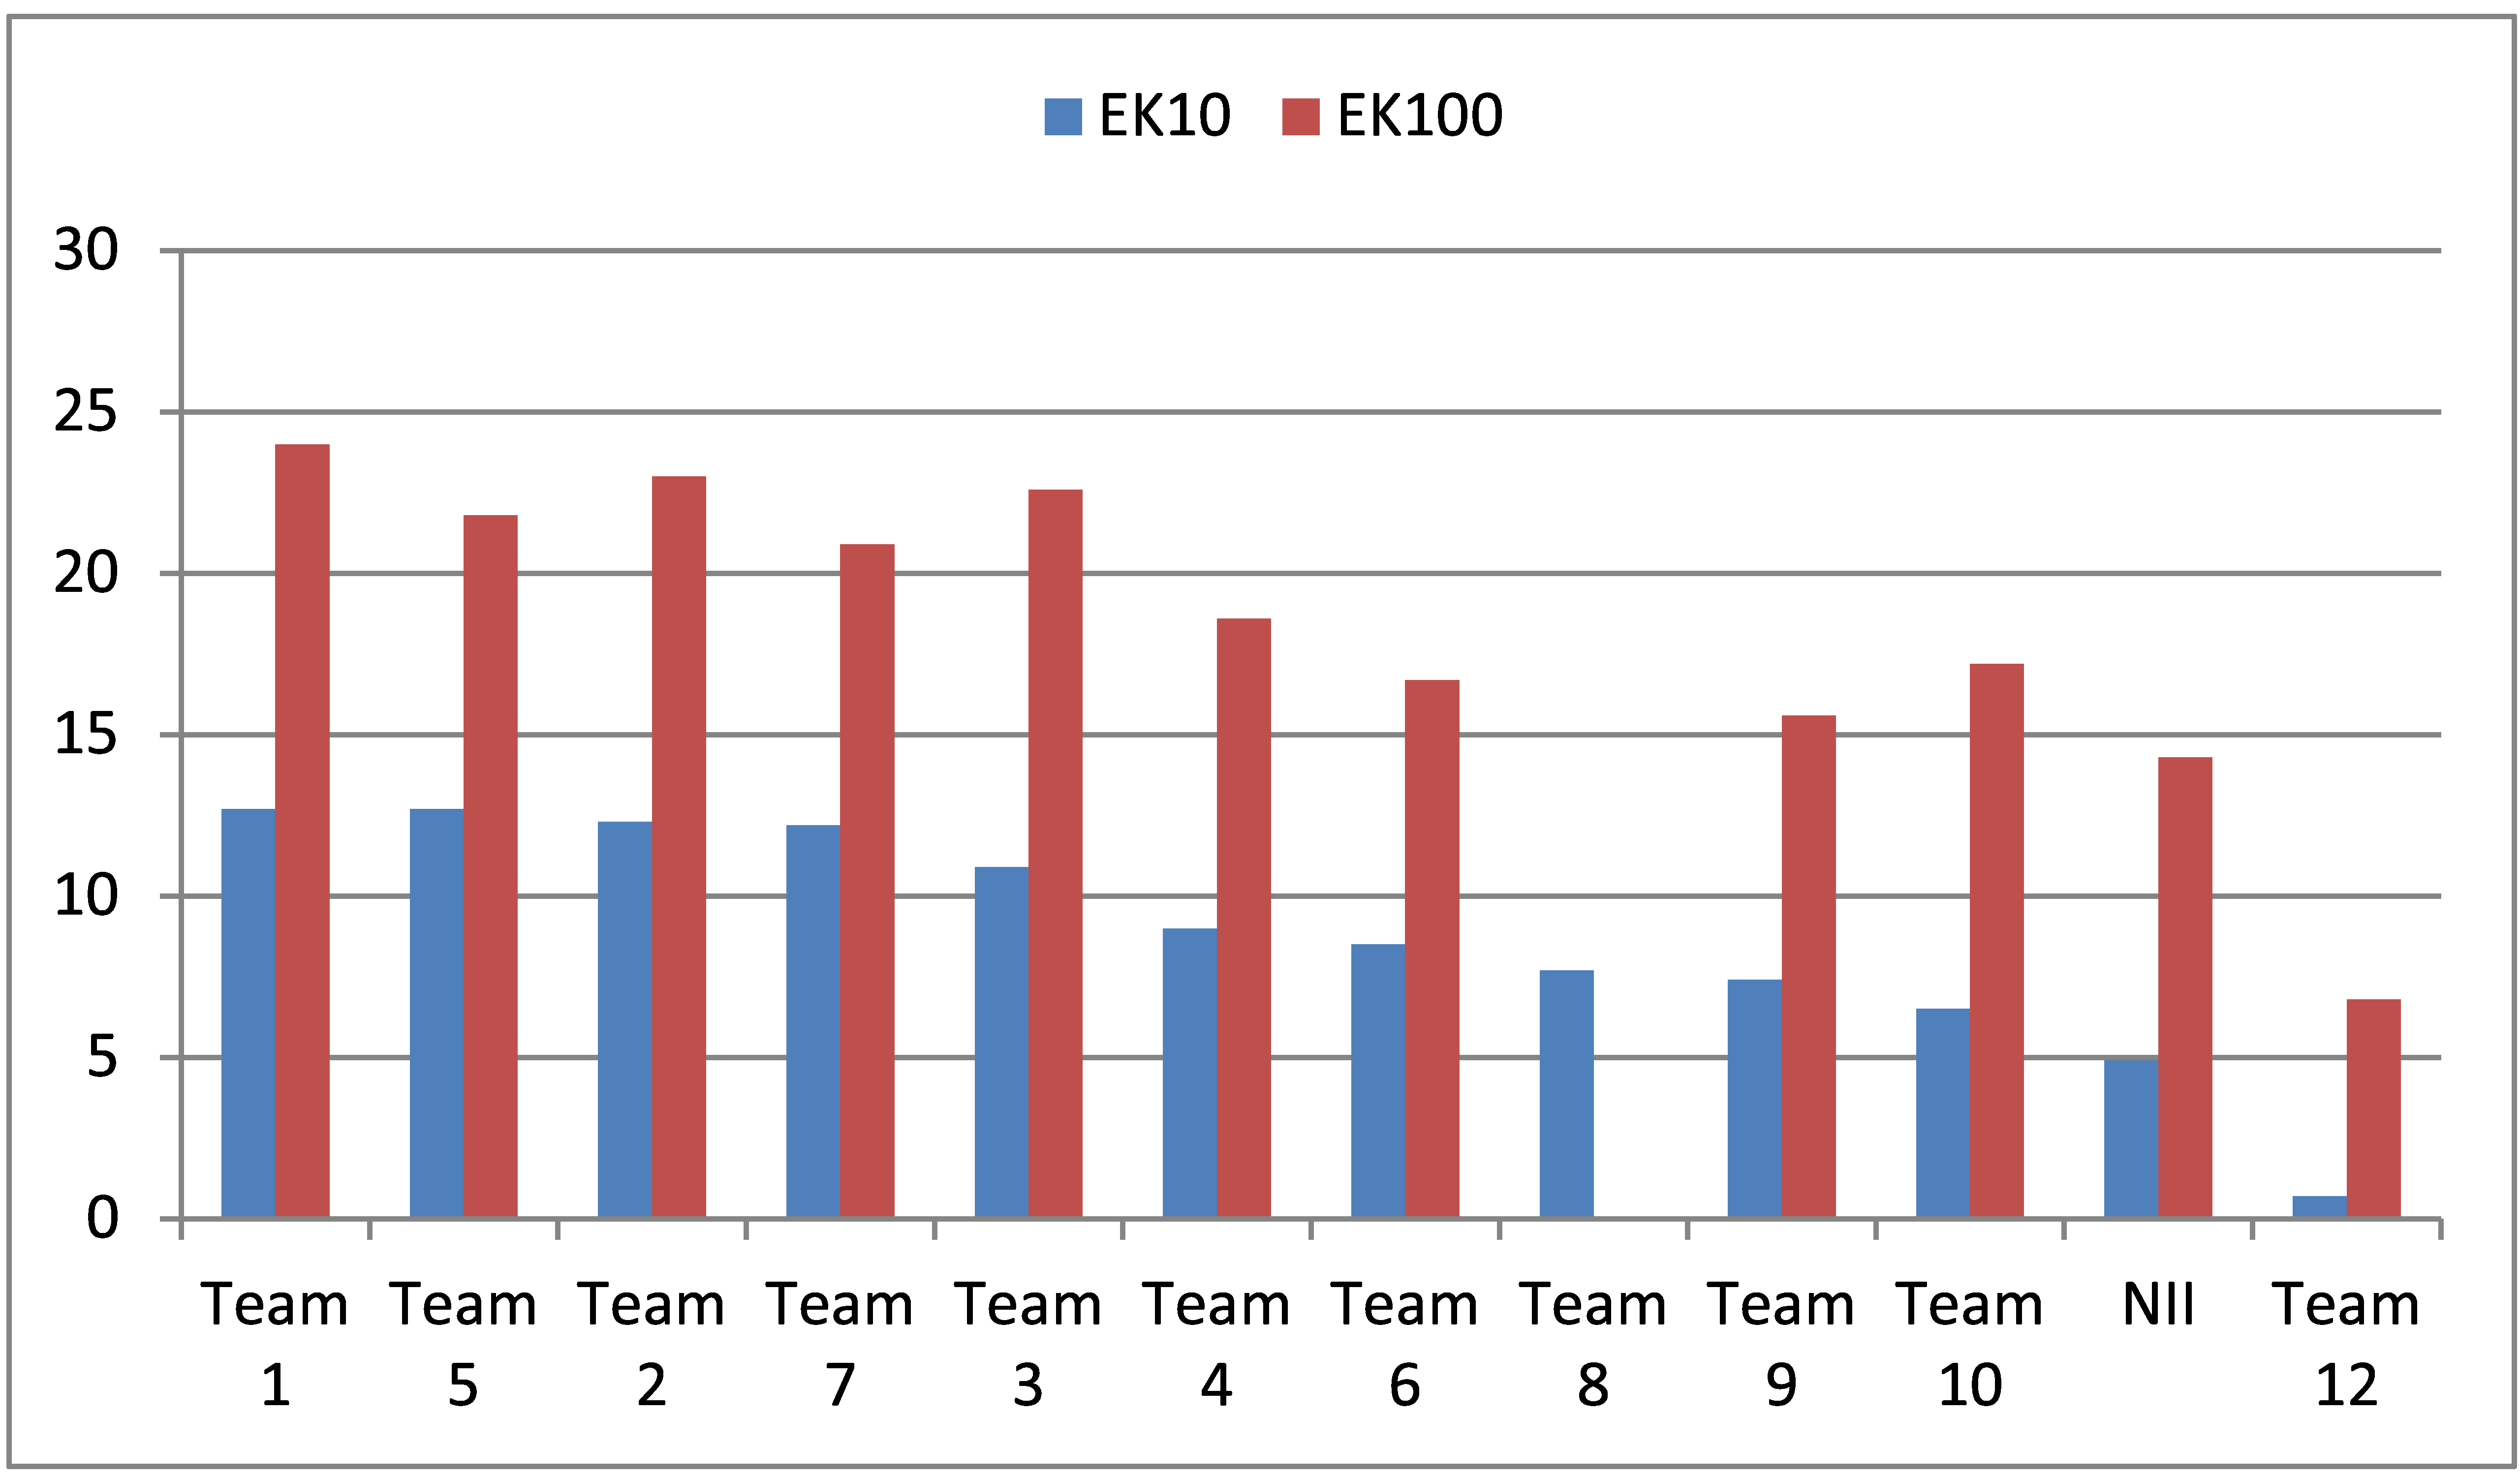
\includegraphics[width=0.7\linewidth]{med_result_ah.pdf}
		\caption{Ad-Hoc Systems}
		\label{fig_result_ah}
	\end{subfigure}
	\caption{Comparison of our MED 2014 system with others on the full evaluation set for both Pre-specified and Ad-hoc tasks. Results are sorted in the descending order of performance on the EK10 setting.}
	\label{fig:results}
\end{figure}


